\documentclass{article}
\usepackage[utf8]{inputenc}
\usepackage[right=.75in, left=1.5in, top=1.25in, bottom=1.25in]{geometry}
\usepackage{setspace}
\usepackage{fancyhdr}
\usepackage{imakeidx}
\usepackage{multirow}
\usepackage{tikz}
\usepackage{hyperref}
\hypersetup{
    colorlinks=true,
    linkcolor=black,
    filecolor=magenta,      
    urlcolor=cyan,
    pdftitle={Overleaf Example},
    pdfpagemode=FullScreen,
    }
    
\title{Práctica 2}
\author{Christian Néstor Barriga Marcapura\\
        Weimar Ccapatinta Huamani}
\date{Agosto 27, 2022}

\begin{document}

\maketitle

\tableofcontents
\newpage
\pagestyle{fancy}
\fancyhf{}
\lhead{Algoritmos y Estructura de datos}
\rhead{Práctica 2}
\chead{UNSA}
\rfoot{\thepage}{}
\section{Introducción}
\doublespacing En ciencias de la computación, un árbol binario es una estructura de datos en la cual cada nodo puede tener un hijo izquierdo y un hijo derecho. No pueden tener más de dos hijos (de ahí el nombre "binario"). Si algún hijo tiene como referencia a null, es decir que no almacena ningún dato, entonces este es llamado un nodo externo. En el caso contrario el hijo es llamado un nodo interno. Usos comunes de los árboles binarios son los árboles binarios de búsqueda, los montículos binarios y Codificación de Huffman.

\section{Estructucturas de datos de árbol}
\doublespacing Se han evaluado los siguientes algoritmos:
\subsection{AVL Tree}
 Fue la primera estructura de datos de este tipo que se inventó. En un árbol AVL, las alturas de los dos subárboles secundarios de cualquier nodo difieren como máximo en uno; si en algún momento difieren en más de uno, se realiza un reequilibrio para restaurar esta propiedad. La búsqueda, la inserción y la eliminación toman tiempo O (log n ) tanto en el promedio como en el peor de los casos, donde{\ estilo de visualización n}nortees el número de nodos en el árbol antes de la operación. Las inserciones y eliminaciones pueden requerir que el árbol sea reequilibrado por una o más rotaciones de árbol .
 
 \center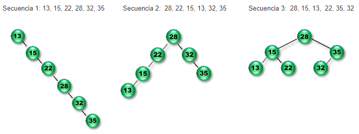
\includegraphics[trim={0.cm 0.cm 0cm 0.cm},clip,scale=1]{Practica 2/niveles AVL.png}
 \center El mismo conjunto de datos, por ejemplo: 13, 15, 28, 32, 35, 22, puede generar con distintas alturas.

 \center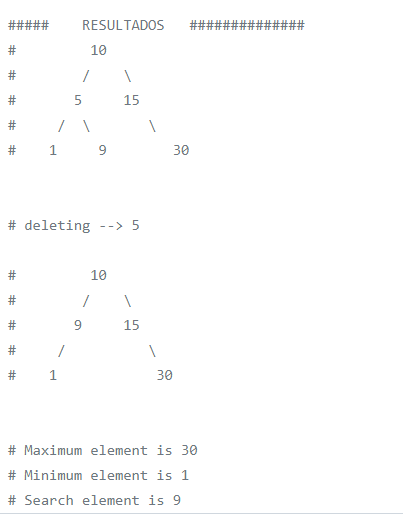
\includegraphics[trim={0.cm 0.cm 0cm 0.cm},clip,scale=1]{Practica 2/AVL1.png}
 \center Figura 1 Resultados algoritmo AVL Tree - Elaboración propia
\newpage\
 
 \begin{flushleft}
\subsection{B tree}
son árboles balanceados de búsqueda, pero cada nodo puede poseer más de dos hijos. Los árboles B mantienen los datos ordenados y las inserciones y eliminaciones se realizan en tiempo logarítmico amortizado.\\
 Dado que se permite un rango variable de nodos hijo, los árboles-B no necesitan rebalancearse tan frecuentemente como los árboles binarios de búsqueda auto-balanceables. Pero, por otro lado, pueden desperdiciar memoria, porque los nodos no permanecen totalmente ocupados. Los límites (uno superior y otro inferior) en el número de nodos hijo son definidos para cada implementación en particular.
 \end{flushleft} 
 \center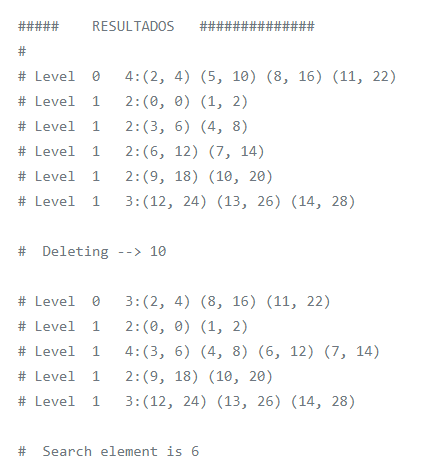
\includegraphics[trim={0.cm 0.cm 0cm 0.cm},clip,scale=1]{Practica 2/b tree.png}
 \center Figura 2 Resultados algoritmo B Tree - Elaboración propia
\newpage\
 \begin{flushleft}
\section{Implementación}
Se envía el siguiente enlace en Github, se ha colocado dos carpetas donde una se encuentra los algoritmos de balance realizados en python y en otra la animación realizada en p5.js.
\url{https://github.com/weicap/MCC_Practica_2}
 \end{flushleft} 
 \center\includegraphics[trim={0.cm 0.cm 0cm 0.cm},clip,scale=0.5]{Practica 2/AVL.png}
 \center Figura 3 Animacion algoritmo AVL Tree - Elaboración propia
\newpage\
  \begin{flushleft}
\section{Conclusiones}
\doublespacing\begin{itemize}
  \item Los árboles AVL son árboles binarios equilibrados que se utilizan principalmente en la indexación de bases de datos.
  \item Todas las operaciones realizadas en los árboles AVL son similares a las de los árboles de búsqueda binarios, pero la única diferencia en el caso de los árboles AVL es que necesitamos mantener el factor de equilibrio, es decir, la estructura de datos debe permanecer como un árbol equilibrado como resultado de varias operaciones. Esto se logra mediante el uso de la operación Rotación de árbol AVL.
  \item Los árboles B tienen ventajas sustanciales sobre otras implementaciones cuando el tiempo de acceso a los nodos excede al tiempo de acceso entre nodos. 

\end{itemize}
\end{flushleft} 
\end{document}

